\documentclass{article}
\usepackage{amsmath} %This allows me to use the align functionality.
                     %If you find yourself trying to replicate
                     %something you found online, ensure you're
                     %loading the necessary packages!
\usepackage{amsfonts}%Math font
\usepackage{graphicx}%For including graphics
\usepackage{hyperref}%For Hyperlinks
\usepackage{listings}
\usepackage{graphicx}
\usepackage{natbib}        %For the bibliography
\bibliographystyle{apalike}%For the bibliography
\usepackage[margin=1.0in]{geometry}
\usepackage{float}
\begin{document}
%set the size of the graphs to fit nicely on a 8.5x11 sheet
\noindent \textbf{Caio Brighenti }\\
\noindent \textbf{COSC 302 - Analysis of Algorithms -- Spring 2019}\\%\\ gives you a new line
\noindent \textbf{Lab 1}\vspace{1em}\\
\begin{enumerate}
	\item Proof \\ 
	A.
		\begin{align}
			a &= b^{log_ba} \\
			log_ba&=log_ba  && \text{definition of log}  \\
			a&=a && \text{simplify}
		\end{align}
	B. \\
		Let $a=c^x$ and $b=c^y$. 
		\begin{align}
			log_c(ab) &= log_c(c^x \cdot c^y) && \text{substitution}\\
			&= log_c(c^{x+y}) && \text{exponent property} \\
			&= x+y && \text{A}\\
			&= log_c(a)+log_c(b) && \text{definition of log}
		\end{align}
		\item Proof \\ 
	C. \\
	Let $a=b^x$ and thus $log_b(a)=x$
		\begin{align}
			log_b(a^n) &= log_b((b^x)^n) && \text{substitution}\\
			&= log_b(b^{xn} && \text{exponent property} \\
			&= xn && \text{A} \\
			&= nlog_b(a) && \text{substitution} 
		\end{align}
	D. \\ 
	Let $log_b(a)=x$
			\begin{align}
			b^x&=a && \text{log definition}\\
			log_c(b^x) &= log_c(a) && \text{multiply both sides by $log_c$} \\
	        xlog_c(b) &= log_c(a) && \text{C} \\
	        x &= \frac{log_c(a)}{log_c(b)} && \text{algebra} \\
	        log_b(a) &= \frac{log_c(a)}{log_c(b)} && \text{substitution} 
		\end{align}
	\item Proof \\ 
	E.
	\begin{align}
		log_b(1/a) &= log_b(1)-log_b(a)&& \text{quotient rule} \\
		&=-log_b(a)  && log_b(1)=0\text{ for any number $b$}  
	\end{align}
	F.
	\begin{align}
		log_b(a)&= \frac{log_a(a)}{log_a(b)} && \text{D} \\
		&= \frac{1}{log_a(b)} && \text{if $a^x=1$, $a$ must equal 1} 
	\end{align}
	\item Proof \\
	G.
	\begin{align*}
		a^{log_bc}&= c^{log_ba} \\
		log_a(a^{log_bc})&= log_a(c^{log_ba}) && \text{multiply both sides by $log_a$} \\
		log_bc &= log_ba \cdot log_ac && \text{A for LHS and C for RHS} \\
		\frac{log_bc}{log_ba} &= log_ac && \text{algebra, true by D} 
	\end{align*}
	\item Proof \\
	H. \\
	\textbf{Claim:} if $f(n)$ and $g(n)$ are monotonically increasing, $f(n)+g(n)$ must also be monotonically increasing.
	\\ We proceed by direct proof. With what we are given, if $n_1<n_2$, it must be by the definition of monotonically increasing that $f(n_1)\leq f(n_2)$ and $g(n_1)\leq g(n_2)$. We start from the second equality and add $g(n_1)$ to both sides:
	$$f(n_1)+g_(n_1)\leq f(n_2)+g(n_1)$$
Since we know that $g(n_1)\leq g(n_2)$, we can substitute on the right hand side and result in:
	$$f(n_1)+g_(n_1)\leq f(n_2)+g(n_2)$$
This precisely meets the definition of monotonically increasing, and matches the function we are trying to prove. Thus, the claim is true.\\\\
	I. \\
	\textbf{Claim:} if $f(n)$ and $g(n)$ are monotonically increasing, $f(g(n))$ must also be monotonically increasing.
	\\ We proceed by direct proof. With what we are given, if $n_1<n_2$, it must be by the definition of monotonically increasing that $f(n_1)\leq f(n_2)$ and $g(n_1)\leq g(n_2)$.  Then if $f(n_1)\leq f(n_2)$ and $g(n_1)\leq g(n_2)$, it must be true that $g(f(n_1))\leq g(f(n_2))$, as can effectively substitute $n_1$ and $n_2$ for $f(n_1)$ and $f(n_2)$ based on the monotonically increasing property of $f(n)$. Thus the claim is true, as $g(f(n_1))\leq g(f(n_2))$ both meets the desired function in the claim and is the exact definition of monotonically increasing.\\\\
	J. \\
	\textbf{Claim:} if $f(n)$ and $g(n)$ are monotonically increasing, and $f(n)$ and $g(n)$ are nonnegative, $f(g(n))$ must also be monotonically increasing.
		\\ We proceed by direct proof. With what we are given, if $n_1<n_2$, it must be by the definition of monotonically increasing that $f(n_1)\leq f(n_2)$ and $g(n_1)\leq g(n_2)$. We start from the second equality and multiply $g(n_1)$ to both sides:
	$$f(n_1)g_(n_1)\leq f(n_2)g(n_1)$$
	It should be noted that the above only holds for nonnegative values of $f(n)$ and $g(n)$, but this is covered in what we are given. Next, as we know $g(n_1)\leq g(n_2)$ for nonnegative values, we can substitute one for another:
	$$f(n_1)g_(n_1)\leq f(n_2)g(n_2)$$
	As in the first case, this both matches the definition of monotonically increasing and the designated function in the claim, thus the claim is true.
	\item Proof \\
	K. \\
	By the definition of the golden ratio, we have that $\phi^i=\frac{1+\sqrt{5}}{2}$, and consequently $\hat{\phi^i}=\frac{1-\sqrt{5}}{2}$. As this proof relates to the Fibonacci sequence, we have two base cases, $F=0$ and $F=1$.\\
	First base case: 
	$$\frac{\phi^0-\hat{\phi^0}}{\sqrt{5}}=\frac{1-1}{\sqrt{5}}=\frac{0}{\sqrt{5}}=0=F_0$$
	Second base case:
	$$\frac{\phi^1-\hat{\phi^1}}{\sqrt{5}}=\frac{\frac{1+\sqrt{5}}{2}-\frac{1-\sqrt{5}}{2}}{\sqrt{5}}=\frac{\frac{2\sqrt{5}}{2}}{\sqrt{5}}=\frac{\sqrt{5}}{\sqrt{5}}=1=F_1$$
	Through the inductive hypothesis, we can assume that:
	$$F_n=\frac{\phi^n-\hat{\phi^n}}{\sqrt{5}}$$
	For all nonegative $n$ less than or equal to $i$. We must then show that the following holds:	
	$$F_{i+1}=\frac{\phi^{i+1}-\hat{\phi^{i+1}}}{\sqrt{5}}$$
	By the definition of the Fibbonaci sequence, we can rearrange:
	$$F_{i+1}=F_i+F_{i-1}=\frac{\phi^i-\hat{\phi^i}}{\sqrt{5}}+\frac{\phi^{i-1}-\hat{\phi^{i-1}}}{\sqrt{5}}$$
	I have been unable to finish the problem from this point. I believe I should either substitute the definition for phi and rearrange, or use exponent rules to rearrange and obtain the equality in the claim, but I have not been able to get this to work.
	\item Proof \\
	The base case for this problem is $i=1$. The result is as follows:
	\begin{align}
	\sum_{i=1}^{1}(-1)^11^2&=\frac{(-1)^11(1+1)}{2} \\
	-1&=-1
	\end{align}
	Therefore the base case holds. By the inductive hypothesis, we assume that the claim is true for $n=k$, and thus want to show that it holds for $k+1$. By the definition of summation, we have that:
	\begin{align}
	\sum^{k+1}_{i=1}(-1)^ii^2&=\sum^{k}_{i=1}(-1)^ii^2+(-1)^{k+1}(k+1)^2 
	\end{align}
	Using the inductive hypothesis, we can then substitute and simplify:
	\begin{align}
	&=\frac{(-1)^kk(k+1)}{2} +(-1)^{k+1}(k+1)^2 && \text{inductive hypothesis}\\
	\end{align}
	I became stuck with this problem as well. I am certain that I am close, and that to finish this proof I would have to rearrange the above expression with algebra to result in:
	\begin{align}
	&=\frac{(-1)^k+1(k+1)^2}{2}
	\end{align}
	\item Proof \\
	We start with the base case $n=1$. The base case is as follows:
	\begin{align}
	\sum_{i=1}^{1}\frac{1}{1(1+1)}&=\frac{1}{1+1}\\
	\frac{1}{2}&=\frac{1}{2}
	\end{align}
	Through the inductive hypothesis, we assume that the claim holds for $n=k$, and thus want to show that it holds for $k+1$. By the definition of summation, we have that:
	\begin{align}
	\sum_{i=1}^{k+1}\frac{1}{i(i+1)}=\sum_{i=1}^{k}\frac{1}{i(i+1)}+\frac{1}{k+1(k+2)}
	\end{align}
	We use the inductive hypothesis to substitute and simplify:
	\begin{align}
	&=\frac{k}{k+1}+\frac{1}{k+1(k+2)} && \text{induction hypothesis} \\
	&=\frac{k(k+2)+1}{(k+1)(k+2)} && \text{algebra} \\
	&=\frac{(k+1)^2}{(k+1)(k+2)} && \text{algebra}\\
	&=\frac{k+1}{k+2} && \text{algebra}
	\end{align}
	Thus, the inductive step is true and consequently the claim is true by induction. \\
	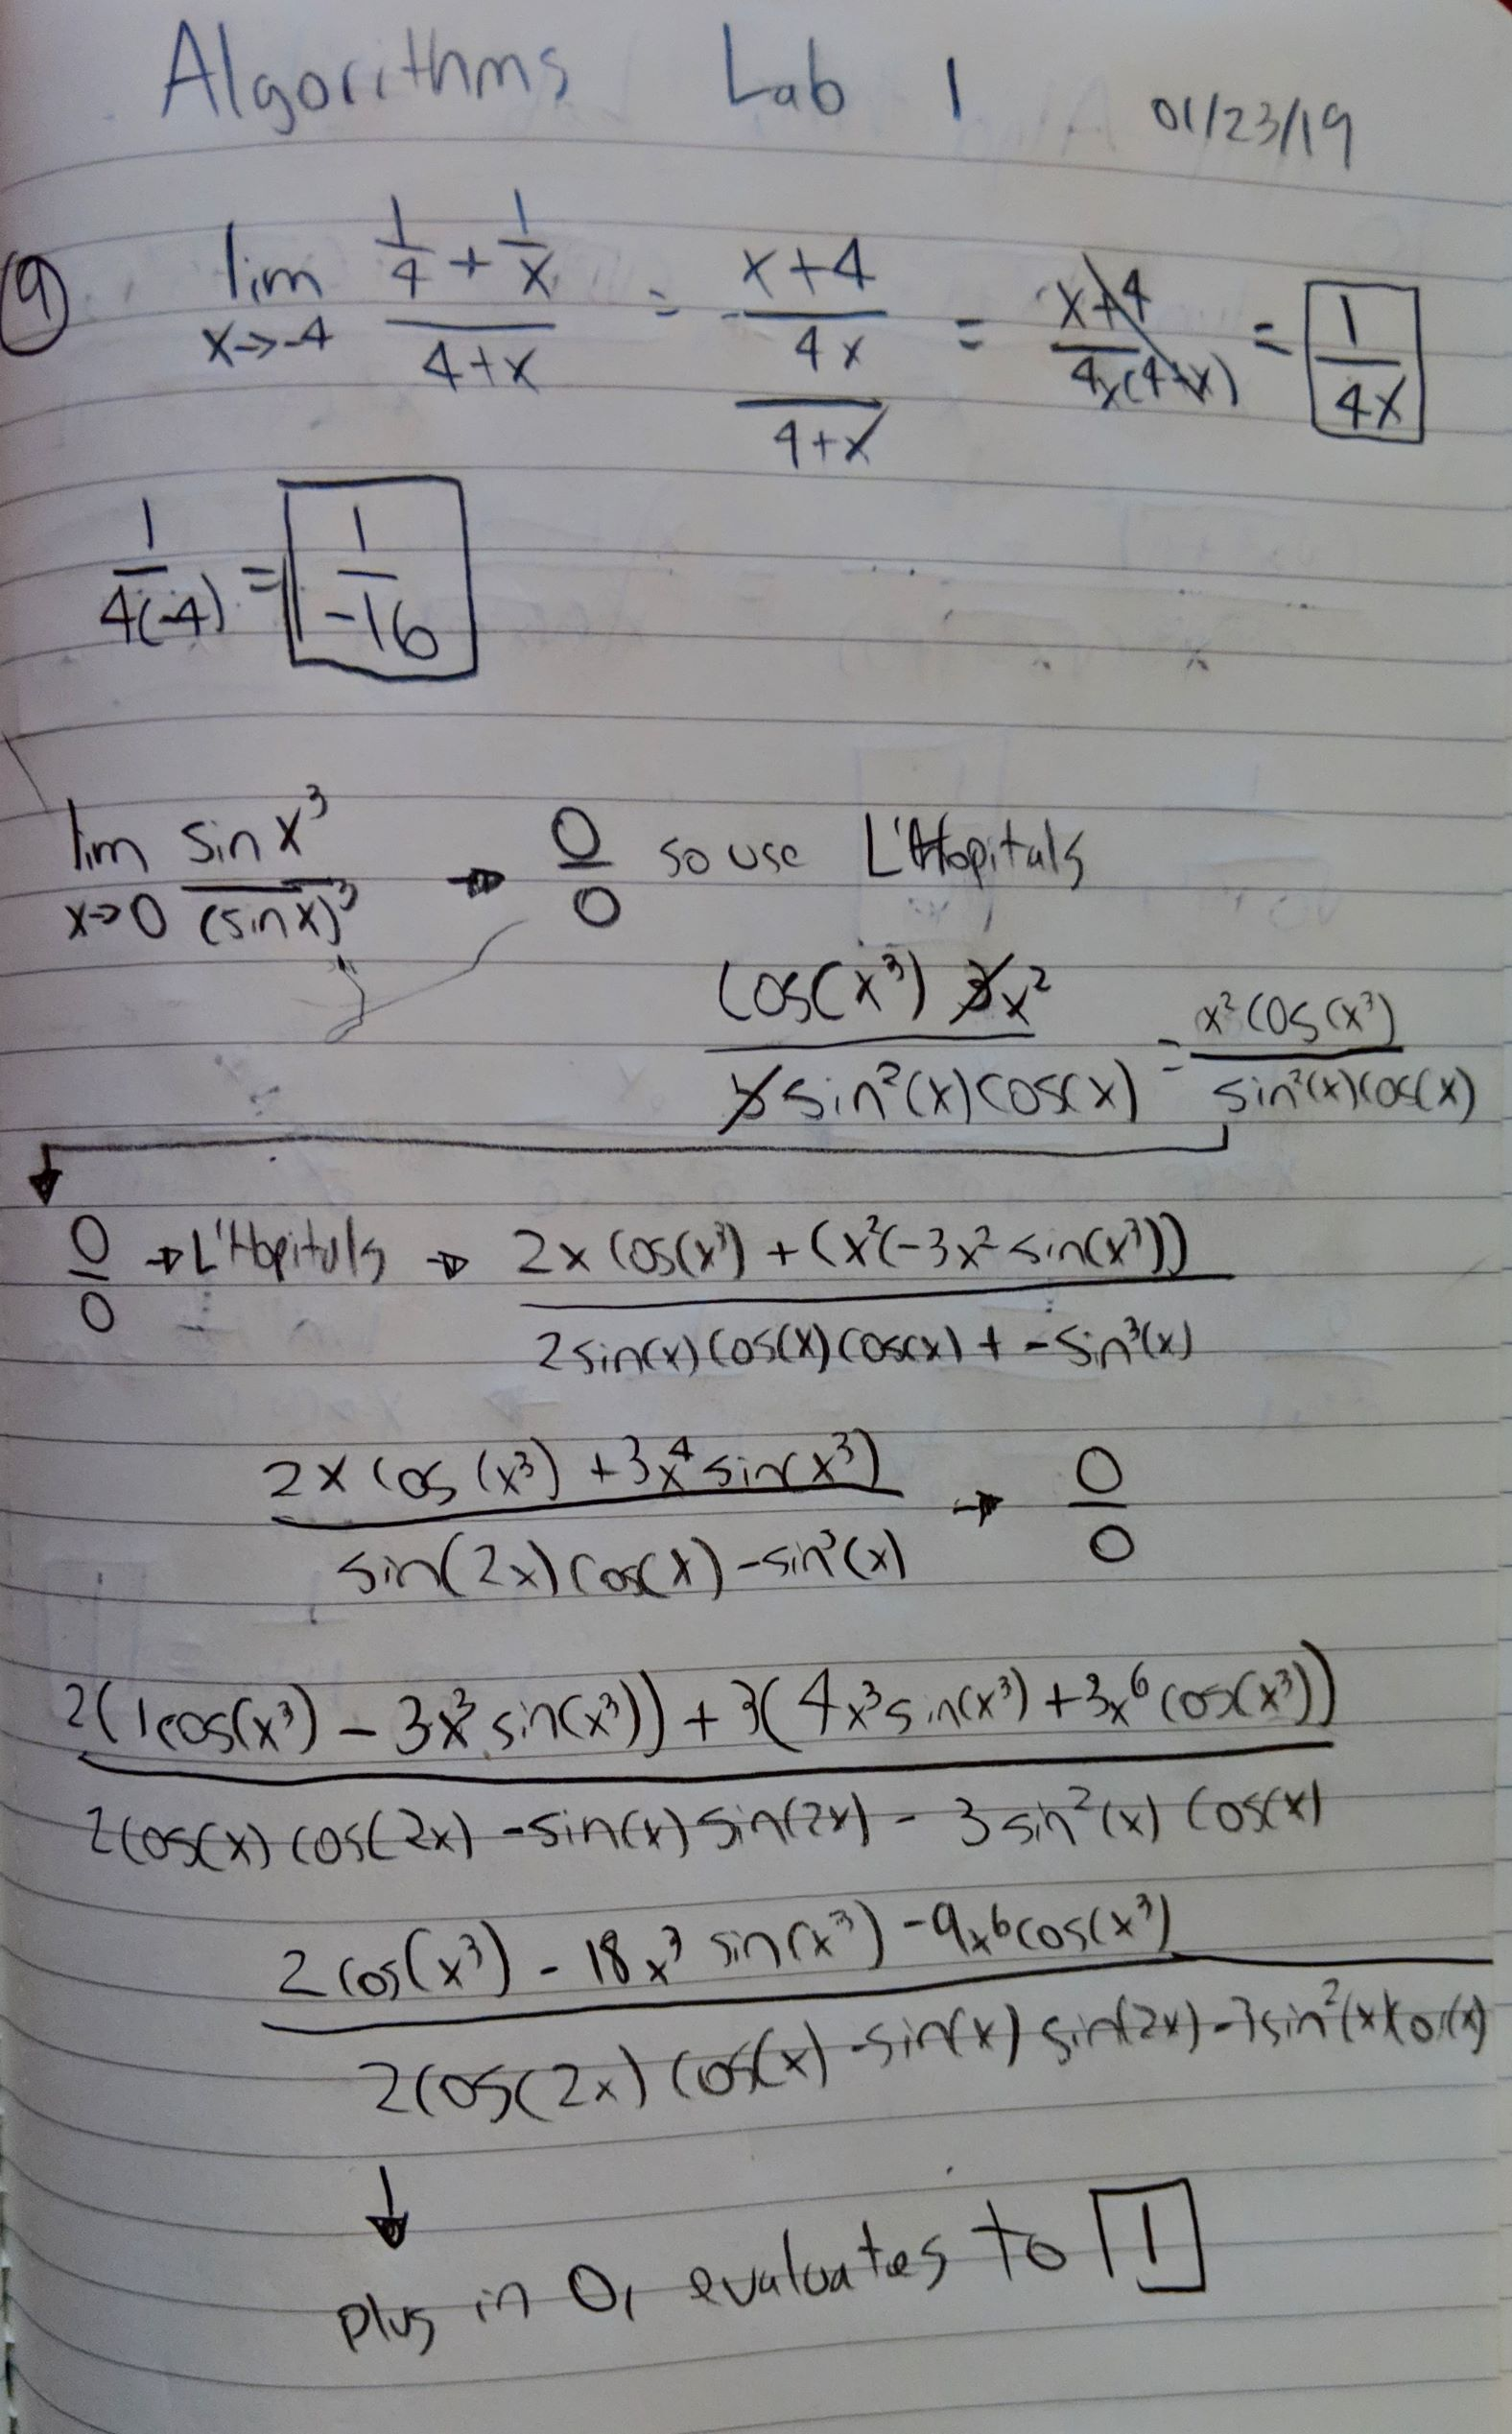
\includegraphics[width=0.85\textwidth]{9_small}\\
	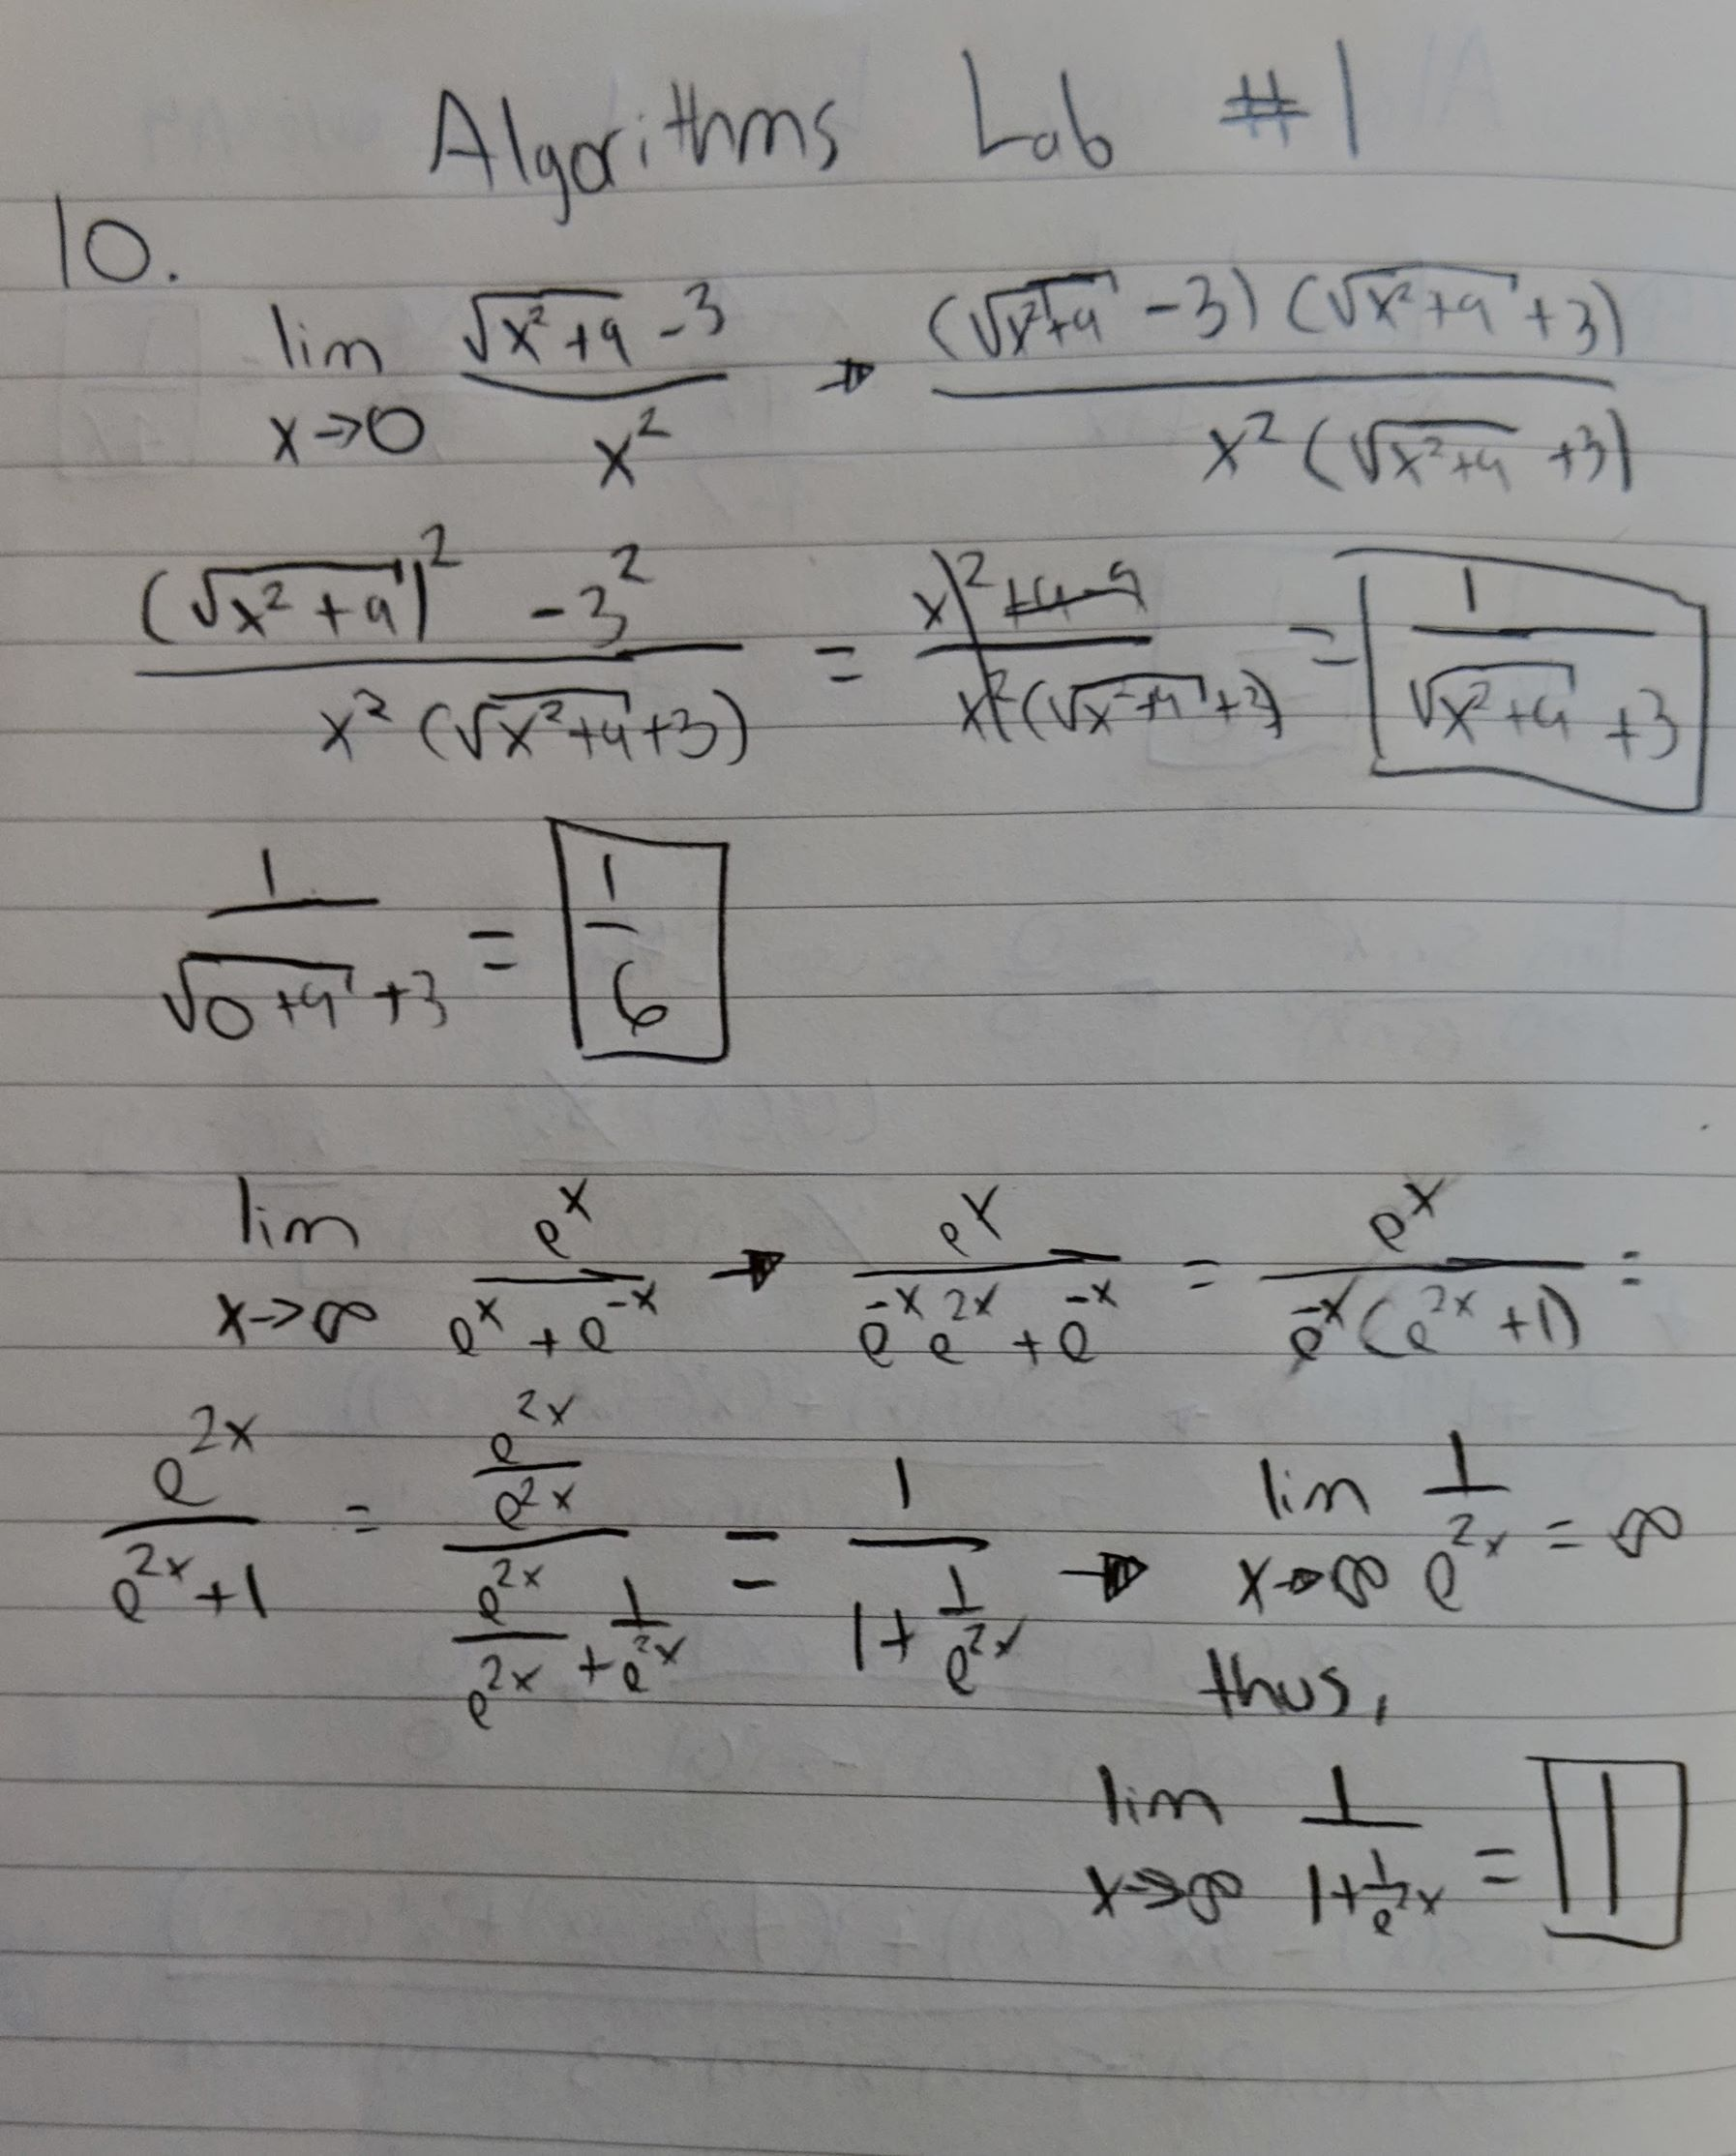
\includegraphics[width=0.85\textwidth]{10_small}
\end{enumerate}


\end{document}
